%%%%%%%%%%%%%%%%%%%%%
%                                             %
%                 Experiment M-3              %
%               g with a pendulum             %
%                                             %
%%%%%%%%%%%%%%%%%%%%%

% Hyperref doesn't like math in chapter titles.
%\iffalse
\labChapter{M}{Fluid Physics with Archimedes’ \& Bernoulli’s Principles}
%\else
%\labChapter{M}{FLUIDS}
%\fi
\label{lab:M08_Fluids}


% Background
\section{Background}

Matter most commonly exists as a solid, liquid, or gas; these states are known as the three common phases of matter. We will investigate liquids in today's experiments. While solids are rigid with specific shapes and definite volumes where molecules are locked in position with their neighbors, liquids and gases are considered to be fluids because they are \textit{not rigid} where the molecules are not locked in place and can therefore flow (i.e. move with respect to each other). 

%If an object is placed in a liquid, the object could displace some of the liquid to either float, sink, or stay somewhere in between. If liquid For ideal fluids (negligible viscosity and incompressible) We can also  were to flow through a given area, 

In today's experiments, we seek to understand why objects float or sink in a liquid (water) using Archimedes Principle regarding fluid statics as well as how liquid flows using Bernoulli's Principle regarding fluid dynamics.


\subsection{Archimedes' Principle}

Archimedes' Principle states: ``When an object is submerged in a fluid, the fluid exerts an upwards buoyant force equal to the weight of the fluid displaced by the object."

%When placed in a fluid, some objects float due to a buoyant force. Where does this buoyant force come from? Does it also act on objects that sink? 

As depth increases, pressure in a fluid increases. Therefore, for an object in a fluid, the upward force on the bottom of that object is greater than the downward force on top of that object (see pressure forces $F_{\text{down}}$ vs $F_{\text{up}}$ in Fig.~\ref{M08_fluids_Fig01} \textit{left}). There is a net upward force, or \textbf{buoyant force}, on any object in any fluid. If the buoyant force is greater than the object’s weight, the object will rise to the surface and float. If the buoyant force is less than the object’s weight, the object will sink (depicted in Fig.~\ref{M08_fluids_Fig01}~\textit{right-a} with $F_\text{Buoyancy} < w_\text{object}$). If the buoyant force equals the object’s weight, the object will remain suspended at that depth. As such, there is always a buoyant force acting on an object regardless of whether it floats, sinks, or remains suspended.

\begin{figure}[ht]
  \begin{center}
    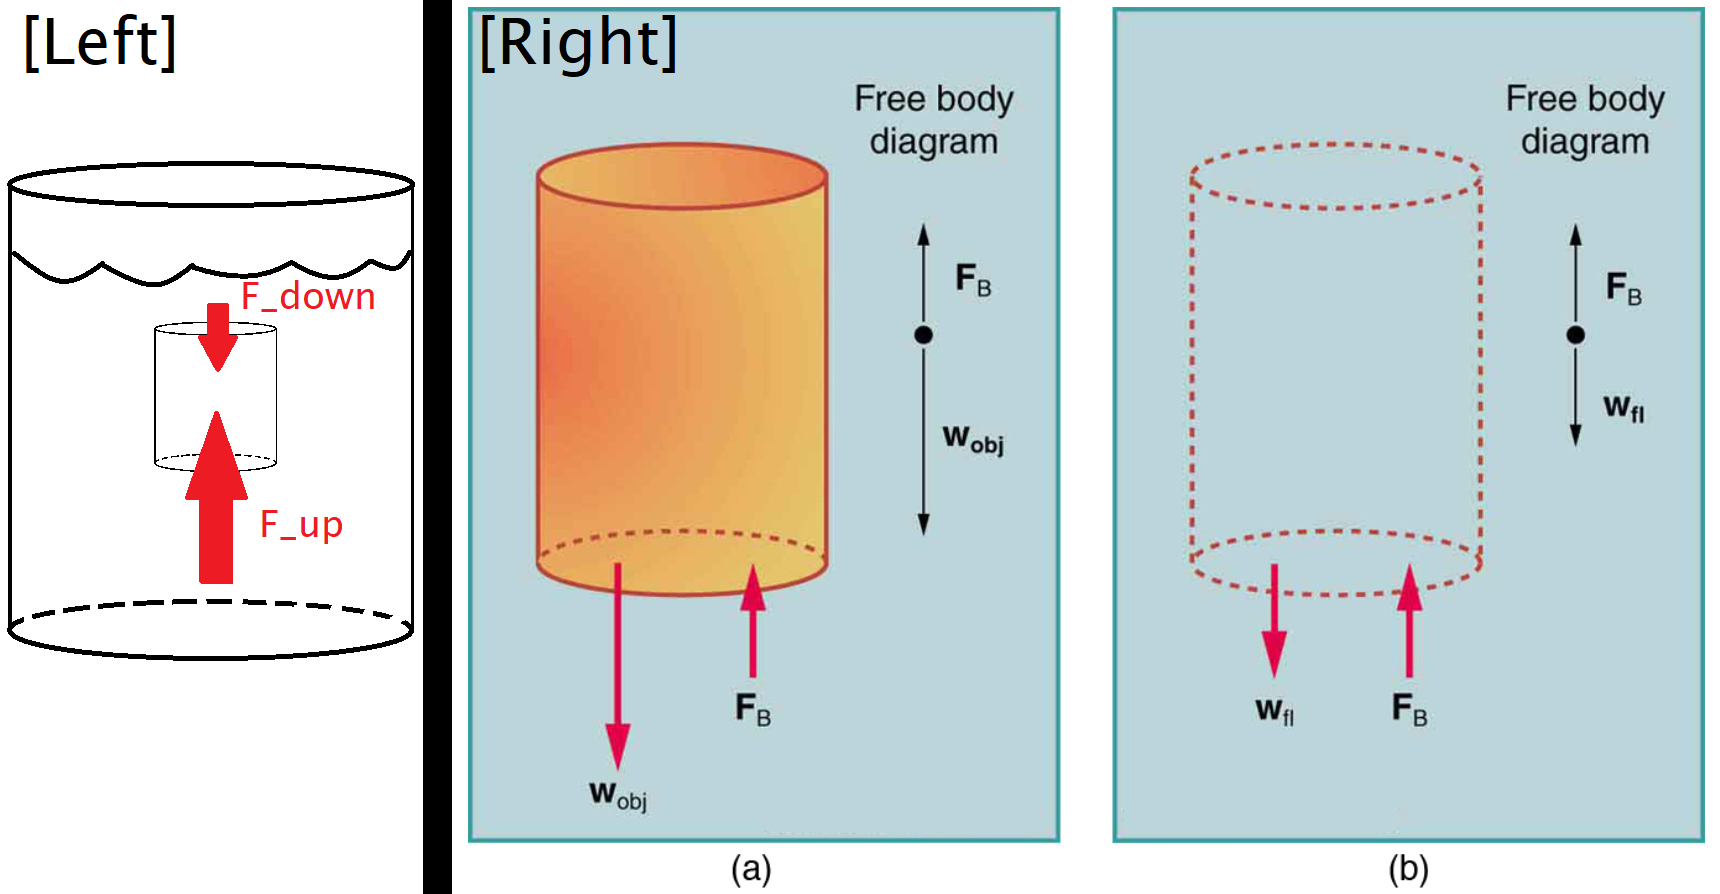
\includegraphics[width=5.3in]{Fall/Experiment08Figures_Fluids/M08_fig00_2.png}
  \end{center}
  \caption{\textbf{\textit{LEFT}}) Pressure due to the weight of a fluid increases with depth causing a greater upward force on the bottom of the object than the smaller downward force on the top of the object. ($F_{\text{down}} < F_{\text{up}}$ and horizontal forces cancel.) \textbf{\textit{RIGHT-a}}) An object submerged in a fluid experiences a buoyant force $F_\text{B}$. If $F_\text{B}$ is greater than the weight of the object $w_\text{obj}$, the object will rise. If $F_\text{B} < w_\text{obj}$ as depicted in \textbf{a}, the object will sink. \textbf{\textit{RIGHT-b}}) If the object is removed, it is replaced by fluid having weight $w_\text{fl}$. Since this weight is supported by surrounding fluid, the buoyant force must equal the weight of the fluid displaced. That is, $F_\text{B} = w_\text{fl}$, a statement of Archimedes’ principle.}
  \label{M08_fluids_Fig01}
  %  \caption{\textbf{\textit{LEFT}}) Pressure due to the weight of a fluid increases with depth since $P=h\rho{}g$. This pressure and associated upward force on the bottom of the cylinder are greater than the downward force on the top of the cylinder. Their difference is the buoyant force $F_\text{B}$. (Horizontal forces cancel.) \textbf{\textit{RIGHT-a}}) An object submerged in a fluid experiences a buoyant force $F_\text{B}$. If $F_\text{B}$ is greater than the weight of the object $w_\text{obj}$, the object will rise. If $F_\text{B} < w_\text{obj}$ as depicted in \textbf{a}, the object will sink. \textbf{\textit{RIGHT-b}}) If the object is removed, it is replaced by fluid having weight $w_\text{fl}$. Since this weight is supported by surrounding fluid, the buoyant force must equal the weight of the fluid displaced. That is, $F_\text{B} = w_\text{fl}$, a statement of Archimedes’ principle.}
\end{figure}

How could we determine the buoyancy force $F_\text{B}$ acting on the object within the fluid? It helps to describe this by removing the object (as in Fig.~\ref{M08_fluids_Fig01}~\textit{right-b}). The volume of the space left behind is filled in by fluid having a weight $w_\text{fl}$. Since that fluid is supported by the surrounding fluid, that weight of the fluid $w_\text{fl}$ (originally displaced by the object) is equal to the buoyancy force $F_\text{B}$. This is \textbf{Archimedes' Principle} --- The buoyant force on an object equals the weight of the fluid it displaces:

\begin{equation}
\label{M08_fluids_Eq01}
    F_\text{B} = w_\text{fl}
\end{equation}


\underline{\textbf{First experiment (Archimedes)}}

In this experiment, we will first determine the mass, volume, and density of 6 objects (see Fig.~\ref{M08_fluids_Fig02}). We will then determine the buoyant force acting on each object using Archimedes' Principle by determining the weight of water each object displaces. Finally, we will determine the buoyant force by measuring the apparent weight of an object.

\begin{figure}[ht]
  \begin{center}
    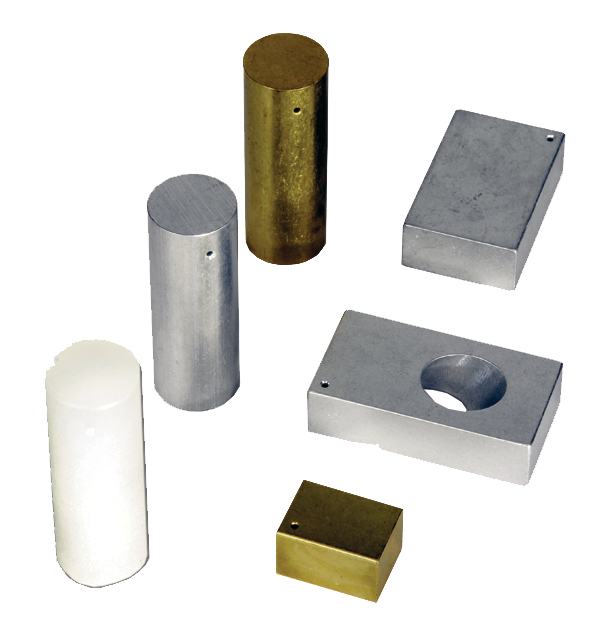
\includegraphics[width=2.9in]{Fall/Experiment08Figures_Fluids/M08_fig02.png}
  \end{center}
%  \caption{3 cylinders (aluminum, brass, plastic), 2 blocks (aluminum, brass), 1 irregular (aluminum).}
  \caption{3 cylinders, 2 blocks, 1 irregular.}
  \label{M08_fluids_Fig02}
\end{figure}

%\underline{\textbf{First experiment, Part I: Mass, Volume, Density}}

As a reminder, the density $\rho$ of an object depends on its mass $m$ and volume $V$:

\begin{equation}
\label{M08_fluids_Eq02}
    \rho = \frac{m}{V}
\end{equation}

and the weight of an object is the downward force due to gravity:

\begin{equation}
\label{M08_fluids_Eq03}
    w_\text{obj} = mg
\end{equation}




\begin{figure}[ht]
  \begin{center}
    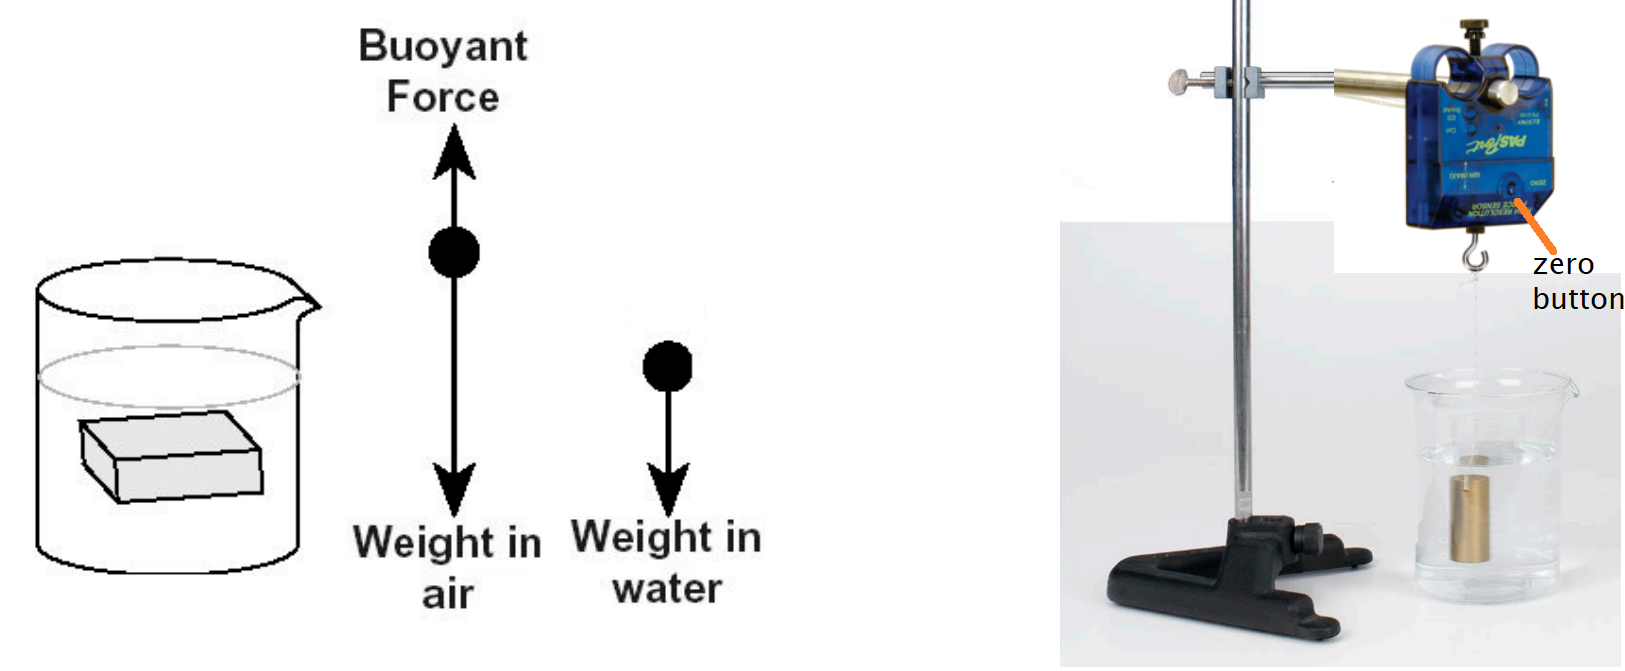
\includegraphics[width=4.9in]{Fall/Experiment08Figures_Fluids/M08_fig06.png}
  \end{center}
%  \caption{3 cylinders (aluminum, brass, plastic), 2 blocks (aluminum, brass), 1 irregular (aluminum).}
  \caption{Left) Force diagram. Apparent weight in water is the difference of weight in air and buoyant force. Right) Force sensor measuring apparent weight of object in water.}
  \label{M08_fluids_Fig04}
\end{figure}

When an object is submerged in a fluid, the apparent weight of the object is less than the weight in air because of the upward buoyant force (see Fig.~\ref{M08_fluids_Fig04}). Thus, the buoyant force can be calculated by finding the difference between the weight of the object in air and the apparent weight of the object when it is submerged in water.

\begin{equation}
\label{M08_fluids_Eq04}
    F_\text{B} = w_\text{obj in air} - w_\text{obj in water}
\end{equation}


%\underline{\textbf{First experiment, Part II: Buoyant Force Using Archimedes' Principle}}
%The buoyant force on several objects is measured by weighing the water displaced by the object as it is submerged. 

%\underline{\textbf{First experiment, Part III: Buoyant Force by Finding the Upward Force}}
%The buoyant force is also determined by measuring the difference between the object's weight in air and its apparent weight in water. Some of the objects have the same density, some have the same volume, and some have the same mass. The density of each object is measured and the dependence of the buoyant force on density, mass, and volume is explored. 

%force sensor rather than lifting the triple beam balance




\subsection{Bernoulli's Principle}

Imagine fluid flowing through a channel of varying width (ex. of such a setup in Fig.~\ref{M08_fluids_Fig07}. As the cross-sectional area changes, the volumetric flow rate remains constant, but the velocity and pressure of the fluid vary.

\begin{figure}[ht]
  \begin{center}
    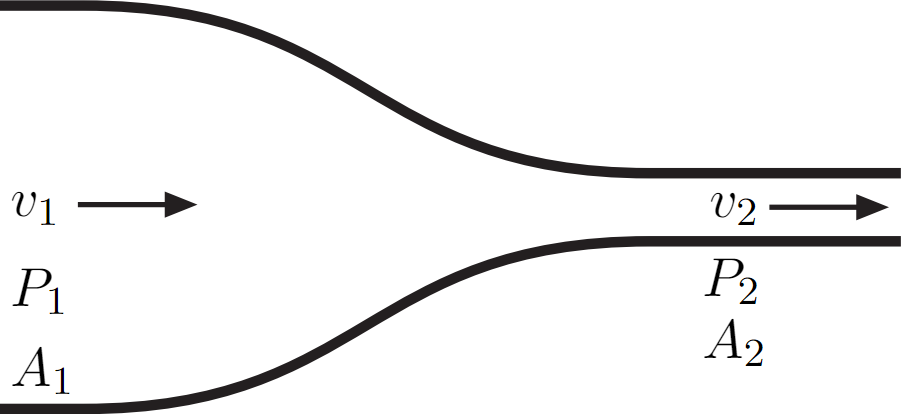
\includegraphics[width=3.9in]{Fall/Experiment08Figures_Fluids/M08_fig07.png}
  \end{center}
  \caption{Example of a Venturi tube, where velocity $v_1 < v_2$, pressure $P_1 > P_2$, and cross-sectional area $A_1 > A_2$}  \label{M08_fluids_Fig07}
\end{figure}

An incompressible fluid of density $\rho$ flows through a pipe of varying diameter. As the cross-sectional area decreases
from $A_1$ (large) to $A_2$ (small), the speed of the fluid increases from $v_1$ to $v_2$. The flow rate, $R = \text{volume}/\text{time}$, of the fluid through the tube is related to the speed of the fluid ($v = \text{distance}/\text{time}$) and the cross-sectional area of the pipe $A$. The flow rate must be constant over the length of the pipe as everything that goes in one side comes out the other end. This relationship is known as the \textbf{Continuity Equation} which can be expressed as:

\begin{equation}
\label{M08_fluids_Eq05}
    R = A_1 v_1 = A_2 v_2
\end{equation}

As the fluid travels from the wide part of the pipe to the constriction, the speed increases from $v_1$ to $v_2$, and the pressure decreases from $P_1$ to $P_2$. This drop in fluid pressure due to fluid speeding up as it flows through a constricted section of a pipe is known as the \textbf{Venturi effect}. This effect can be created with the use of a Venturi tube which allows an incompressible fluid to flow from a wider to narrower section with minimal turbulence.

Assuming the path an incompressible fluid takes is frictionless with no viscous forces, then the energy of the fluid is conserved. The fluid can be analyzed by the total work done on the fluid from the initial position to final position within the tube (total change in both kinetic and potential energy). The full derivation is in your lecture textbook, but for now, we arrive at \textbf{Bernoulli's Equation}. For an \textbf{incompressible, frictionless fluid}, the combination of pressure and the sum of kinetic and potential energy densities is \textit{constant} not only over time, but also along a streamline:

\begin{equation}
\label{M08_fluids_Eq06}
    P + \frac{1}{2}\rho v^2 + \rho g y = \text{constant}
\end{equation}

Note the similarities in Eqn.~\ref{M08_fluids_Eq06} to our previous labs' equations for kinetic and potential energies ($\frac{1}{2}m v^2$ \& $m g h$). Applying this to our Venturi tube of Fig.~\ref{M08_fluids_Fig07}:

\begin{equation}
\label{M08_fluids_Eq07}
    P_1 + \frac{1}{2}\rho v_{1}^2 + \rho g y_1 = P_2 + \frac{1}{2}\rho v_{2}^2 + \rho g y_2
\end{equation}

However, since our tube will be horizontal, we can remove the height dependence and our pressure change is due only to the velocity change (noted by the Continuity Equation in Eqn.~\ref{M08_fluids_Eq05}). Thus, our equation simplifies to \textbf{Bernoulli's Principle} of fluid flow at a \textbf{constant height}:

\begin{equation}
\label{M08_fluids_Eq08}
    P_1 + \frac{1}{2}\rho v_{1}^2 = P_2 + \frac{1}{2}\rho v_{2}^2
\end{equation}


Rearranged another way to determine the pressure at the constriction:

\begin{equation}
\label{M08_fluids_Eq08}
    P_2 = P_1 - \frac{1}{2}\rho (v_{2}^2 - v_{1}^2)
\end{equation}


\underline{\textbf{Second experiment (Bernoulli)}}

In our experiment, we will assume we don't know the pressure at the constriction $P_2$, and will use the Continuity and Bernoulli equations to determine theoretically what $P_2\text{ theoretical}$ should be and compare to the actual value $P_2\text{ actual}$ as measure by our pressure sensor.

The setup will be as in Fig.~\ref{M08_fluids_Fig08}. Water can be released from the pitcher sitting on the white/plexiglass box with the cooler-style spout as the release valve. On the other end of the water hose will be a hose clamp for use during the determination of the flow-rate to rapidly stop the flow of water (if you only used the spout at the pitcher, much of the water would continue flowing out of the tube even after shutting if off, messing up the flow-rate calculations). 

$P_1$, as measured by the Quad Pressure Sensor, will be treated as a known actual or accepted value to be used in our calculations to solve for $P_{2\text{ theoretical}}$. It will be connected to port 1 (or port 3 if in the future these sensors break). 

We will calculate $P_{2\text{ theoretical}}$ from our Continuity and Bernoulli equations. The value of $P_{2\text{, actual}}$, as measured by the Quad Pressure Sensor, will be treated as the known actual value to compare to. $P_2$ will be connected to port 2 (or port 4 if sensor is damaged). 

NOTE: The pressure sensor hoses are to have only (or mostly) air such that water does not reach the pressure sensor. To avoid water getting up the air hoses, ensure the Venturi tube is positioned with the air hoses pointed upward. After passing through the Venturi tube, the water will flow into a catch basin. There will also be a stopwatch to measure flow-rate during the first part of the experiment.

If you require more water in your pitcher, use another pitcher to refill (assuming the catch basin is glass, there will be less of a chance of that breaking if we're not moving it around more than we have to).




\begin{figure}[ht]
  \begin{center}
    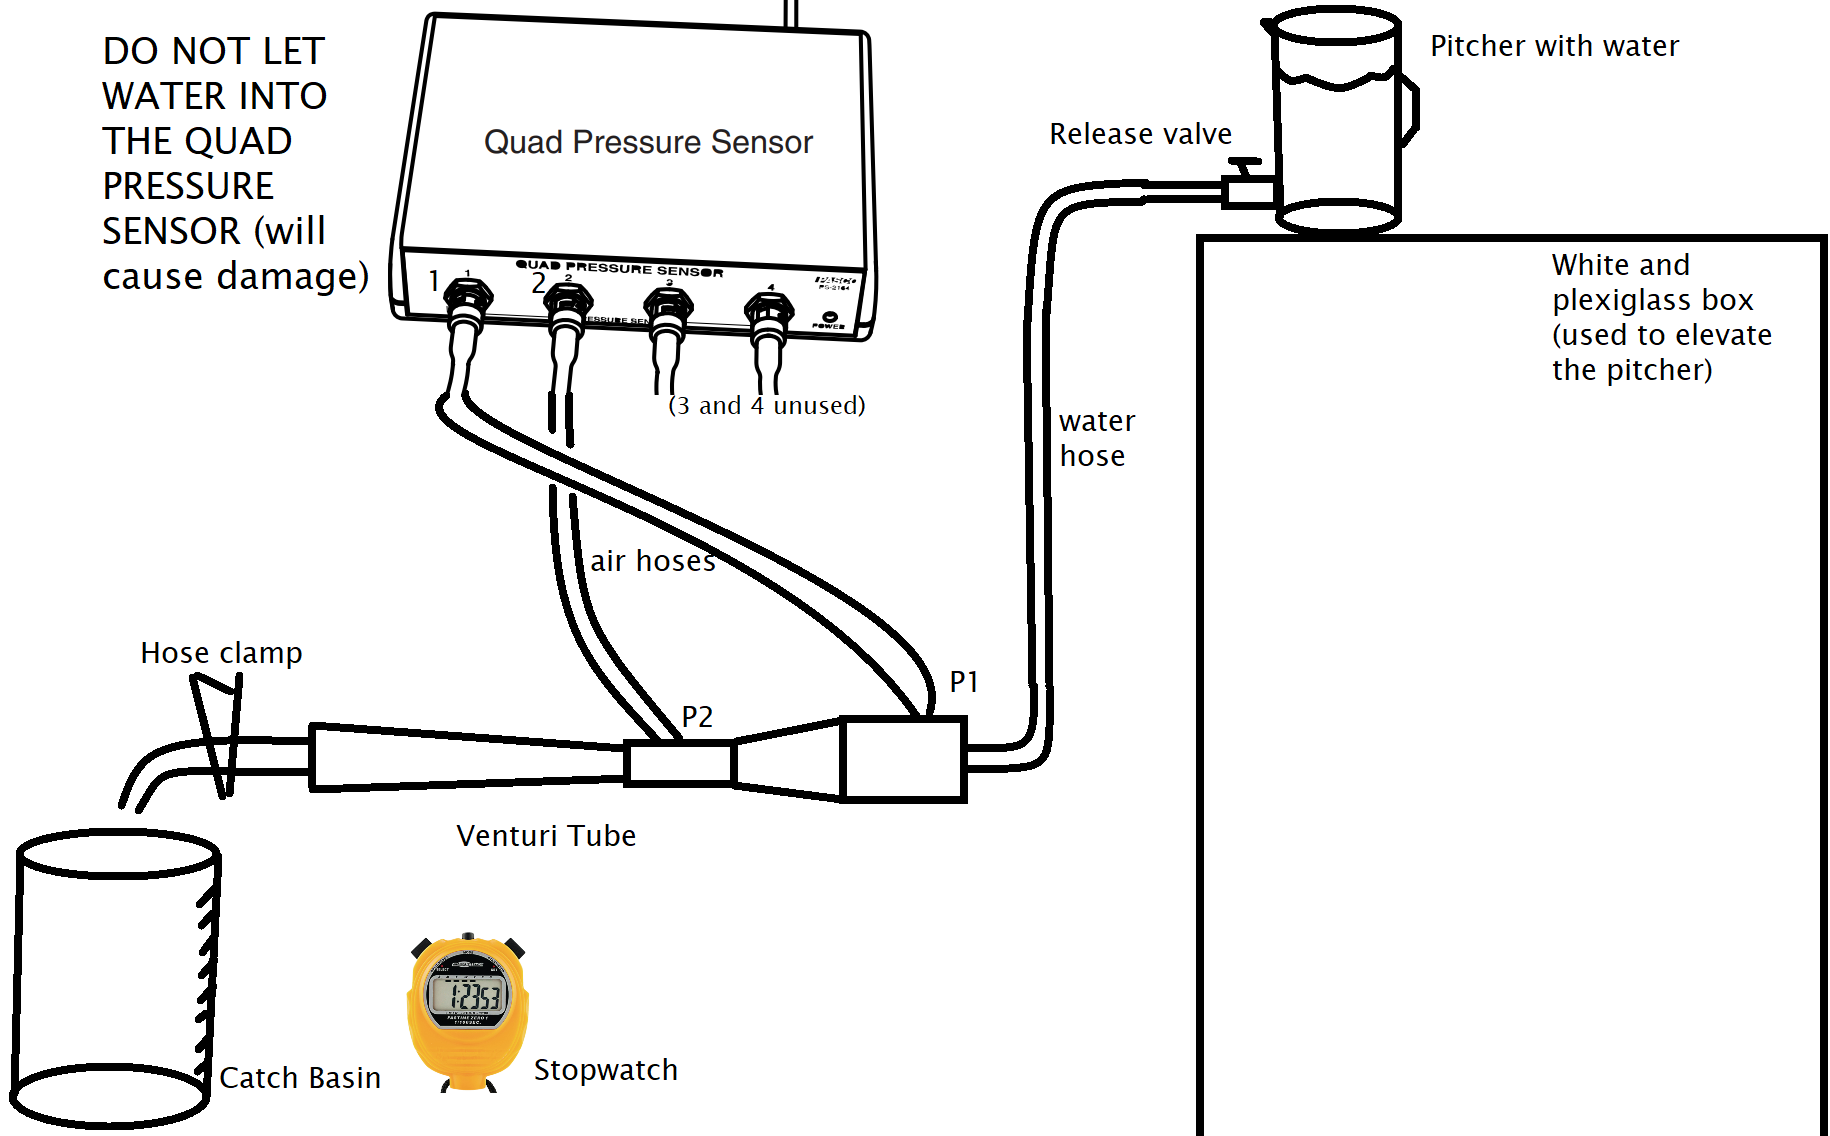
\includegraphics[width=5.9in]{Fall/Experiment08Figures_Fluids/M08_fig08.png}
  \end{center}
  \caption{Sketch of the Venturi tube setup for the second experiment (Bernoulli).}
  \label{M08_fluids_Fig08}
\end{figure}










\section{Experimental Procedure}


\subsection{Archimedes' Principle (First experiment)}

\begin{enumerate}

\item \textbf{OVERALL GOALS:} 
\begin{itemize}
    \item Understand the relationship between buoyancy force and the mass, volume, density of an object.
    %\item Assume \textbf{we know the resistance} of your resistors, but \textbf{we don't know the capacitance} of the capacitors, and we need to determine those C values.
    \item Determine buoyant force using Archimedes' Principle.
    \item Determine buoyant force by measuring the upward force directly.
    %\item Understand  \textit{DISCUSSION POINT}: 
\end{itemize}


\underline{\textbf{Part I: Mass, Volume, and Density}}

\item Create a data table with:
\begin{itemize}
    \item Columns for the mass $m$, relevant dimensions (length, width, height, radius), volume $V$, and density $\rho$
    \item Rows for each of the 6 objects (clearly label or describe the objects in the table).
\end{itemize} 

\item Using the triple-beam balance, find the mass of each of the six objects. List the objects in order from least to greatest mass. \textit{Consider: are any of the masses nearly the same?}

\item Using the calipers, measure the dimensions of the 3 cylinders and the 2 blocks (Fig.~\ref{M08_fluids_Fig03}). Remember to divide the diameter by 2 to get the radius, $r$. Calculate the volume $V$ of these objects %(can use cm$^3$ to be consistent with the irregular shape in the next step). 
$V_\text{cylinder} = \pi r^2 h$ and $V_\text{block} = lwh$

\item There is no simple formula for the volume of the irregularly shaped object, so it is necessary to find the volume by measuring the volume of water it displaces:
\begin{itemize}
    \item Put the beaker under the overflow can spout as shown in Fig.~\ref{M08_fluids_Fig03}.
    \item Pour water into the overflow can until it overflows into the beaker. Allow the water to stop overflowing on its own and empty the beaker into your pitcher and return it to its position under the overflow can spout without jarring the overflow can.
    \item Tie a string on the irregular object.
    \item Gently lower the irregular object into the overflow can until it is completely submerged. Allow the water to stop overflowing and then pour the water from the beaker into the graduated cylinder. Measure the volume of water that was displaced by reading the water level in the graduated cylinder in milliliters (1 ml = 1 cm$^3$)
\end{itemize}

\begin{figure}[ht]
  \begin{center}
    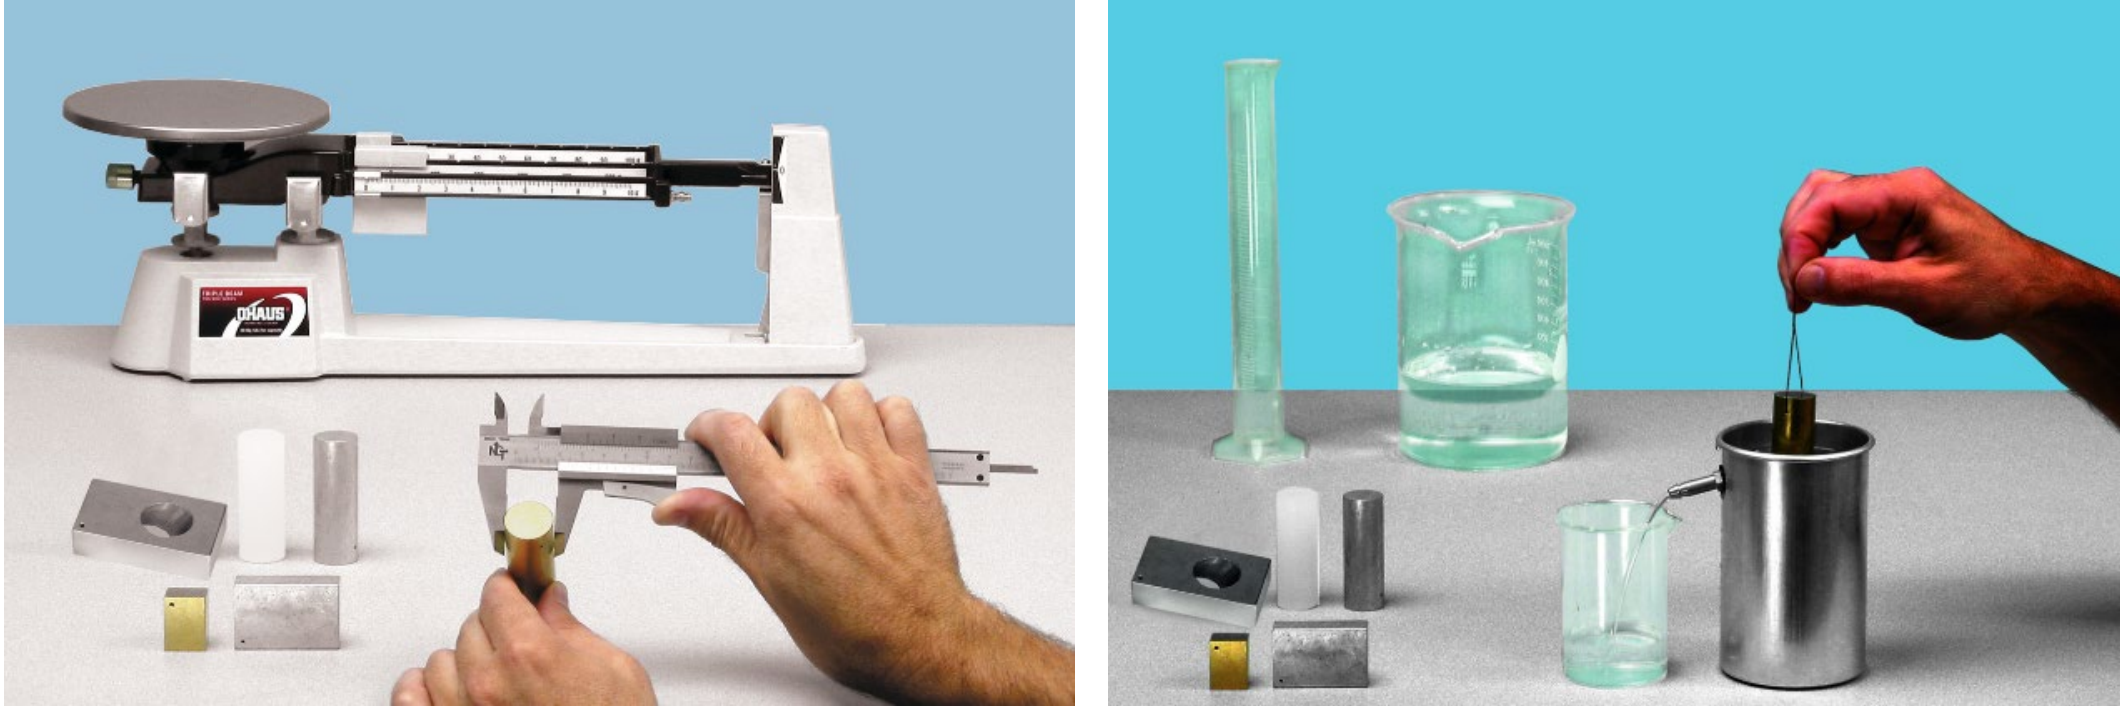
\includegraphics[width=4.9in]{Fall/Experiment08Figures_Fluids/M08_fig03.png}
  \end{center}
  \caption{Left) Measuring with calipers. Right) Lowering object into overflow can.}
  \label{M08_fluids_Fig03}
\end{figure}

\item List the 6 objects in order from least to greatest volume. \textit{Consider: Is this the same order as the mass list? Are any of the volumes nearly the same?}

\item Calculate the density of each object. List the 6 objects in order from least to greatest density. \textit{Consider: Is this list in the same order as either the mass list or the volume list? Do any of the objects have densities that are nearly the same?}

\item Group the objects according to the type of material of which they are made. \textit{Consider: In which list (mass, volume, or density) are the objects grouped similarly?}

%\item Create a data table:



\underline{\textbf{Part II: Finding the Buoyant Force Using Archimedes' Principle}}

For each of the objects, find the weight of the water displaced by each one:

\item Create a data table with:
\begin{itemize}
    \item Mass of beaker and other common data
    \item Columns for the mass $m_\text{water} = m_\text{total} - m_\text{beaker}$, weight $w_\text{water} = m_\text{water} g = F_\text{B}$
    \item Rows for each of the 6 objects plus a half-submerged brass cylinder (so 7 rows). Clearly label or describe the objects in the table.
\end{itemize} 
\item Find the mass of the beaker. Put the beaker under the overflow can spout as shown in Fig.~\ref{M08_fluids_Fig03}.
\item Pour water into the overflow can until it overflows into the beaker. Allow the water to stop overflowing on its own and empty the beaker into the pitcher and return it to its position under the overflow can spout without jarring the overflow can.
\item Tie a string onto each of the objects.
\item Gently lower the first object into the overflow can until it is completely submerged. Allow the water to stop overflowing. Find the mass of the water plus beaker. Subtract the mass of the beaker to determine the mass of the displaced water. Multiply the mass by the acceleration due to gravity (9.803 m/s$^2$) to find the weight of the water.
\item Repeat this procedure for the other objects. Note that the plastic cylinder will float so don’t try to completely submerge it in the water. Also find the weight of the displaced water when only half the brass cylinder is submerged.
\item List the objects in order from least buoyant force to greatest buoyant force. \textit{Consider: Is this in the same order as the mass list, the volume list, or the density list? Are any of the buoyant forces nearly the same? Why or why not?}


\underline{\textbf{Part III: Finding the Buoyant Force by Finding the Upward Force}}

\item Create a data table:
\begin{itemize}
    \item Seven rows for each of the 6 objects as well as the brass cylinder half-submerged (clearly label or describe the objects in the table).
    \item Columns for weight in air $w_\text{obj in air}$, apparent weight in water $w_\text{obj in water}$, buoyant force $F_\text{B}$ as determined with Eqn.~\ref{M08_fluids_Eq04}.
\end{itemize}
\item Tie a loop on the other end of the string so it can be hooked onto the force sensor.
\item In Capstone, press record or monitor, and you will see the force in Newtons displayed (constantly updating). You can let this continue running to act as a continuous scale.
\item Before hanging any of the objects on the force sensor hook, zero the force sensor with the physical ``zero" button on the front of the force sensor (shown in Fig.~\ref{M08_fluids_Fig04}).
\item With the water out of the way, record the weight of each object in air $w_\text{air}$ by hanging them on the hook. 
\item Zero the sensor as needed if it appears to be drifting when swapping out the different objects.
\item Now place the pitcher of water beneath the force sensor such that when you hang each object from the force sensor hook, the objects can be fully submerged. Record the apparent weight of each object in water $w_\text{water}$.
\item Calculate the buoyant force for each object by taking the difference between the weight in air and the weight in water (Eqn.~\ref{M08_fluids_Eq04}).
\item Add an additional column and calculate for each object case the \% difference between the buoyancy force (found here by measuring the upward force) and the buoyancy force found previously by Archimedes' Principle of the displaced water. 

$\% \text{ diff.} = \frac{F_\text{B, upward force method} - F_\text{B, Archimedes' method}}{F_\text{B, Archimedes' method}} \times 100$ 

\textit{Consider: In each case, is the buoyant force that was determined using the upward force equal to the
weight of the water displaced?}



\end{enumerate}





\subsection{Bernoulli's Principle (Second experiment)}

\begin{enumerate}

\item \textbf{OVERALL GOALS:} 
\begin{itemize}
    \item Understand fluid-flow continuity through different constrictions.
    %\item Assume \textbf{we know the resistance} of your resistors, but \textbf{we don't know the capacitance} of the capacitors, and we need to determine those C values.
    \item Determine flow-rate of our system using the Continuity Equation.
    \item Understand Bernoulli's Principle of fluid flow at a constant height to investigate the Venturi effect and determine the pressure of a fluid at a constriction point (in a Venturi tube).
    %\item Understand  \textit{DISCUSSION POINT}: 
\end{itemize}


\underline{\textbf{Part I: Determining Flow Rate $R$}}
\item Create a data table:
\begin{itemize}
    \item 6 rows for five trials of the measuring flow rate as well as the average flow rate $R_\text{avg}$ and standard deviation of your flow rate $\sigma_R$.
    \item Columns for the volume $\Delta V$ of water, elapsed time $\Delta t$ it took to flow, and flow rate $R$.
\end{itemize}
    \item With water in the pitcher, open the release-valve (spout) to allow water to flow and remove most of any air bubbles within the tubing. After a couple seconds, tighten the hose clamp at the end to halt the flow. Take whatever water is in the catch basin and return it to the pitcher.
    \item Start current trial with the catch basin empty.
    \item Start the stopwatch and open the hose clamp at the same time to start water flow.
    \item After a measurable amount of water has flowed through, stop the stopwatch and close the hose clamp at the same time.
    \item Measure the volume of water that flowed out of (or into) the apparatus (either with the scale on the catch basin or graduated cylinder).
    \item Calculate the average flow rate for the current trial $R = \frac{\Delta V}{\Delta t}$ where $\Delta V$ is the volume of water and $\Delta t$ is the elapsed time.
    \item Empty the catch basin or graduated cylinder back into the pitcher to keep a consistent amount of water in it.
    \item Rerun this process starting with the empty catch basin (assuming the water hose is still clear of air bubbles) 4 more times for a total of 5 trials.
    \item From the individual trial flow rates, calculate the average flow rate $R_\text{avg}$ and standard deviation $\sigma_R$ which we will use to represent our uncertainty in the flow rate ($R_\text{avg} \pm \sigma_R$).
    \item NOTE: Typically the flow rate varies with the level of water in the reservoir. To keep the flow rate close to constant, make the pressure measurements with the water level approximately the same as it was for the flow rate measurement.



\underline{\textbf{Part II: Determining Pressure at a Constriction}}

\hspace{6mm}\underline{\textbf{with Continuity and Bernoulli Eqns.}}

\item Create a data table:
\begin{itemize}
    \item Common data section including:
    \begin{itemize}
        \item Flow rate $R_\text{avg} \pm \sigma_R$ from Part I.
        \item Cross-sectional areas $A_1$ and $A_2$ and their uncertainties $\delta_{A_1}$ and $\delta_{A_2}$.
        \item Velocities $v_1$ and $v_2$. Also include the max values for each (Used to estimate pressure uncertainty later).
        \item Density of water $\rho$ (use 1000 kg/m$^3$)
    \end{itemize}

    \item 7 rows for five trials of the measuring $P_1$ and $P_2$ in Capstone as well as their averages $P_{1\text{ avg actual}}$ and $P_{2\text{ avg actual}}$ and standard deviations $\sigma_{P_{1\text{ avg actual}}}$ and $\sigma_{P_{2\text{ avg actual}}}$.
    \item Columns for $P_1$ and $P_2$.
\end{itemize}

    \item Determine the cross-sectional areas of the wide and narrow constrictions ($A_1$ and $A_2$ respectively) with the calipers from the cutaway version of the Venturi tubes ($A = \pi r^2$). Note your uncertainty due to your measurement precision ($\delta_{A_1}$ and $\delta_{A_2}$).
    \item Calculate $v_1$ and $v_2$ with the Continuity Eqn.~\ref{M08_fluids_Eq05} based on your measured areas and average flow rate. Similarly, calculate $v_{1\text{ max}}$ and $v_{2\text{ max}}$ by maximizing the flow rate ($R_\text{avg} + \sigma_R$) and minimizing the areas (e.g. $A_1 - \delta_{A_1}$).

\item Capstone will be set up to show two pressures representing $P_1$ and $P_2$. Double check the the pressure taps of the Venturi tube are appropriately connected like in Fig.~\ref{M08_fluids_Fig08} where Channel 1 is connected to the wider part of the Venturi tube, and Channel 2 to the narrow constriction of the Venturi tube. (It'll be easier to keep track of which pressure is which when the labels are similar.) 
\item Capstone will also show a plot with both $P_1$ and $P_2$ on the y-axis as a function of time on the x-axis. To analyze either data set later on, you can click directly on the plotted data.
\item Calibrate the pressure sensor by:
\begin{itemize}
    \item Ensure both the hose clamp and release valve (spout) are closed.
    \item Disconnect the air hoses from the Quad Pressure Sensor via the quick connectors so the pressure sensors are open to atmospheric pressure. Set the air hoses on top of the white box (or in a bracket to hold them if I get them prepared in time) so the end of the hose is above the spout water level to prevent water from siphoning through the air hoses.
    \item In Capstone, select the green Calibration tab on the left-hand panel.
    \item 1) Pressure 2) Select all ``Pressure Measurements" 3) Type of Calibration as ``One Standard (1 point offset)" 4) Set Standard Value to average atmospheric pressure of 101.3 kPa --- Click the "Set Current Value to Standard Value" button 5) Finish
    \item Both Absolute Pressure Channels 1 and 2, when you press record, should now read at about 101.3 kPa, if not, retry the calibration.
\end{itemize}
\item Ensure no water is near the end of the air hoses to prevent any water getting into the pressure sensors. Reconnect the air hoses to the pressure sensors.
\item You can open the hose clamp at the end of the hose as it will not be needed for the rest of this experiment. You will just need to catch basin to collect the water and avoid making a mess.
\item Press record, then open the release valve to allow the water to flow into the catch basin. After any air bubbles have passed and the water is flowing with minimal turbulence, continue recording pressure data for $\sim$5~seconds, then close the release valve (spout) and stop recording.
\label{M08_fluids_BernoulliStep_00}
\item Find the section of your Pressure vs. Time plot where flow was laminar (smooth without bubbles), should be a generally flat section of the Pressure vs Time plot. Click on the $P_1$ data on the plot, enable the highlight tool, and select a chunk of the plot when flow was laminar (no bubbles, the flat part). Do the same for the $P_2$ data. You can find the average value for $P_1$ and $P_2$ at the bottom of the table on the left hand side of your screen, where the mean is representing the average value of whichever subset of the data you've highlighted.
\item Record both $P_{1\text{ actual}}$ and $P_{2\text{ actual}}$. There should be a difference of $\sim 2 \text{--} 5$kPa, if not, double check with an instructor.
\item Rerun this process from Step~\ref{M08_fluids_BernoulliStep_00} an additional 4 times for a total of 5 trials.
\item Determine the $P_{1\text{ avg actual}}$ and $P_{2\text{ avg actual}}$ values from your five trials. Also determine their standard deviations $\sigma_{P_{1\text{ avg actual}}}$ and $\sigma_{P_{2\text{ avg actual}}}$.
\item Calculate your theoretical value of $P_{2\text{ theoretical}}$ with Eqn.~\ref{M08_fluids_Eq08} using your previously determined velocities $v_1$ and $v_2$ and your average $P_{1\text{ avg actual}}$ treated as the known actual value for the wider part of the Venturi tube.
\item Similarly calculate your max theoretical value of $P_{2\text{, max theoretical}}$ by maximizing ${P_{1\text{ avg actual}}}$ (e.g. ${P_{1\text{ avg actual}}} + \sigma_{P_{1\text{ avg actual}}}$) and using your already determined maximized velocities $v_{1\text{ max}}$ and $v_{2\text{ max}}$.
\item Represent your uncertainty $\delta P_{2\text{ theoretical}}$ with the difference of your maximized value and average values (e.g. $\delta P_{2\text{ theoretical}} = P_{2\text{, max theoretical}} - P_{2\text{ theoretical}}$).
\item \textit{Consider:} Does you theoretical value for $P_2$ agree with the actual value of $P_2$ as measured with the pressure sensor?



















    
\end{enumerate}











%\pagebreak

\section{Post-Lab Submission --- Interpretation of Results}

\subsection{Archimedes' Principle (First experiment)}
\begin{itemize}
\item Make sure to submit your finalized data table (Excel sheet)

    \item First Experiment (Archimedes' Principle)
\begin{itemize}
    \item In which list (mass, volume, or density) are the objects grouped similarly?
    \item In each object case, is the buoyant force that was determined using the upward force (Part III) equal to the
weight of the water displaced (Part II)? Were the \% differences between the two methods for each case relatively small, or did any case standout?
    \item Which objects had the same buoyant force when submerged? Why?
    \item For the plastic cylinder, what was the apparent weight in water? What would be the buoyant force be if plastic cylinder were completely submerged?
    \item How did the buoyant force for the totally submerged brass cylinder relate to the buoyant force for the half-submerged brass cylinder?
    \item What does the buoyant force depend on: The mass of the object, or its volume, or its density, or the material from which it is made?
\end{itemize}


    \item Second Experiment (Bernoulli's Principle)
\begin{itemize}
    \item Does you theoretical value for $P_2$ agree with the actual value of $P_2$ as measured with the pressure sensor? \newline (i.e. $P_{2\text{ theoretical}} \pm \delta P_{2\text{ theoretical}}$ overlap with $P_{2\text{ avg actual}} \pm \sigma P_{2\text{ avg actual}}$?)
    \item How is the Bernoulli Principle different than the Bernoulli Equation?
    \item What assumptions about the fluid allows the Bernoulli Principle to work? (i.e. what type or characteristics of the fluid and/or flow are necessary assumptions for Bernoulli to hold true?)
    \item Imagine that instead of being on the table, the Venturi tube were set on the floor with the rest of the experimental apparatus unchanged. Would the difference in pressures we see on the Capstone plot between $P_1$ and $P_2$ during the smooth, laminar flow section that we analyzed to find average pressures be \textit{larger}, \textit{smaller}, or \textit{the same}. Why?
\end{itemize}


    

\end{itemize}